\section{Ejercicio 7: Dise\~no de contadores sincr\'onicos y asincr\'onicos de 3 bits}

\subsection{Contador Asincr\'onico}
En esta secci\'on se propone el dise\~no de un contador asincr\'onico de 3 bits ascendente empleando \'unicamente Flip Flops D, puesto que es el \'unico tipo de Flip Flop del cual se dispone.

\subsubsection{Dise\~no del circuito}
Cada uno de los Flip Flop's corresponder\'a a un bit del contador, y para ser asincr\'onico, cada uno tiene como se\~nal de clock el complemento del bit inferior en peso, salvo el bit menos significativo cuyo clock
corresponde a una se\~nal cuadrada efectivamente. De esta forma, cada vez que se produce un cambio de estado alto a estado bajo en un bit del contador, el siguiente en peso invertir\'a su estado.
Se agrega adem\'as la posibilidad de reiniciar el contador empleando la entrada asincr\'onica de reset. Se puede observar el circuito l\'ogico resultante en la Fig. \ref{fig:contador_asincronico_circuito}.

\begin{figure}[H]
    \centering
        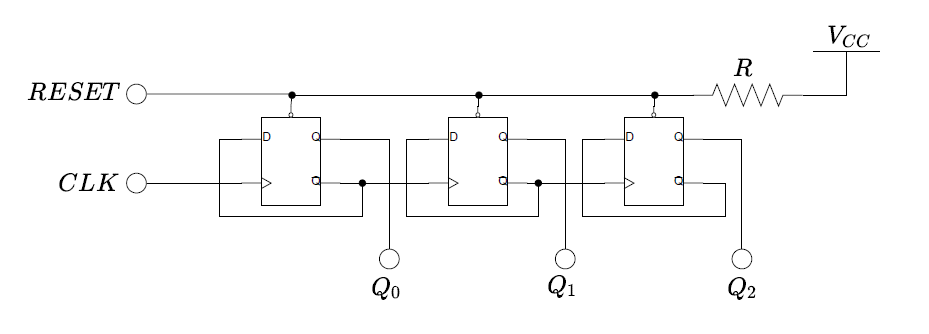
\includegraphics[scale=0.5]{../EJ7/Recursos/contador_asincronico.png}
    \caption{Circuito contador asincr\'onico de 3 bits}
    \label{fig:contador_asincronico_circuito}
\end{figure}

En la pr\'actica se dispone de los circuitos integrados 74LS74, el cual contiene dos flip flops D independientes y necesita tener una tensi\'on de alimentaci\'on de $5V$.
Se conectan sus entradas de preset a $5V$, y luego las entradas asincr\'onicas de reset con un pull-up de $R = 100k\Omega$ a $5V$ para ofrecer al usuario la posibilidad de reiniciar el contador.

\subsubsection{Dise\~no de PCB}

\begin{figure}[H]
    \centering
        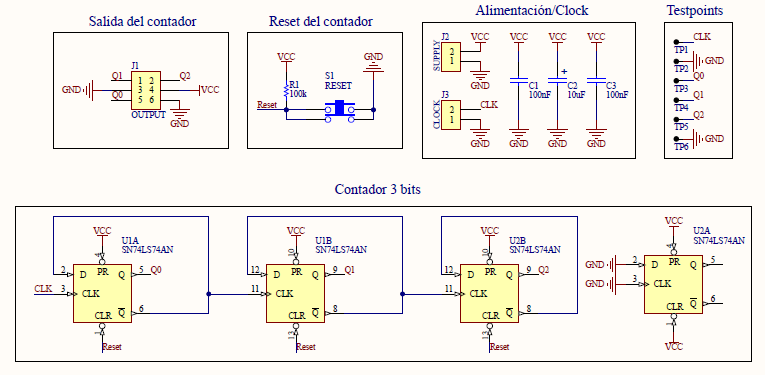
\includegraphics[scale=0.7]{../EJ7/Recursos/esquematico_asincronico.PNG}
    \caption{Esquem\'atico del PCB en Altium Designer}
    \label{fig:esquematico_asincronico}
\end{figure}

\begin{figure}[H]
    \centering
    \begin{tabular}{c c}
        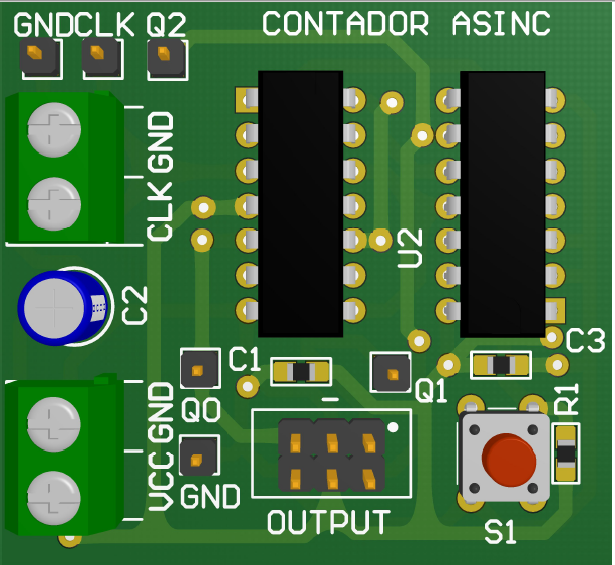
\includegraphics[scale=0.45]{../EJ7/Recursos/3d_top_asincronico.PNG} &
        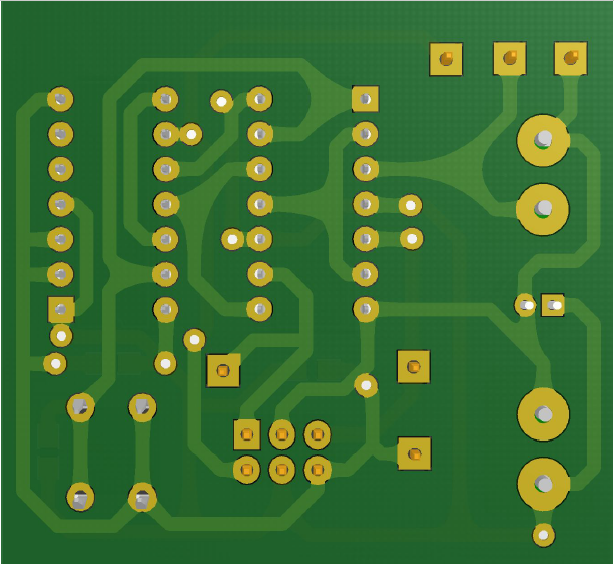
\includegraphics[scale=0.45]{../EJ7/Recursos/3d_bottom_asincronico.PNG} 
    \end{tabular}
    \caption{Dise\~no 3D del PCB}
    \label{fig:3d_asincronico}
\end{figure}

\subsection{Contador Sincr\'onico}
En esta secci\'on se propone el dise\~no de un contador sincr\'onico de 3 bits ascendente empleando \'unicamente Flip Flops D, por la misma raz\'on que para el caso asincr\'onico.

\subsubsection{Dise\~no del circuito}
Para el circuito l\'ogico del contador se propone utilizar los flip flops como dispositivos que almacenen el estado de cada bit del contador,
luego utilizando l\'ogica externa se define c\'omo debe cambiar el estado para cada caso seg\'un el estado actual. Para ello se ilustra en la Tabla. \ref{table:tabla_verdad_contador}
la tabla de verdad del mismo. Entonces se pueden obtener las siguientes expresiones l\'ogicas:

\begin{equation}
    Q^{*}_0 = \neg Q_0 
\end{equation}

\begin{equation}
    Q^{*}_1 = Q_1 \oplus Q_0 
\end{equation}

\begin{equation}
    Q^{*}_2 = Q_2 \oplus (Q_1 \cdot Q_0) 
\end{equation}

\begin{table}[H]
    \centering
    \begin{tabular}{c c c | c c c}
        $Q_2$ & $Q_1$ & $Q_0$ & $Q^{*}_2$ & $Q^{*}_1$ & $Q^{*}_0$ \\ 
        \hline \\
        $0$ & $0$ & $0$ & $0$ & $0$ & $1$ \\
        $0$ & $0$ & $1$ & $0$ & $1$ & $0$ \\
        $0$ & $1$ & $0$ & $0$ & $1$ & $1$ \\
        $0$ & $1$ & $1$ & $1$ & $0$ & $0$ \\
        $1$ & $0$ & $0$ & $1$ & $0$ & $1$ \\
        $1$ & $0$ & $1$ & $1$ & $1$ & $0$ \\
        $1$ & $1$ & $0$ & $1$ & $1$ & $1$ \\
        $1$ & $1$ & $1$ & $0$ & $0$ & $0$ \\
    \end{tabular}
    \caption{Tabla de verdad estados actuales y futuros del contador}
    \label{table:tabla_verdad_contador}
\end{table}

Finalmente, se puede observar la implementaci\'on de estas expresiones en el circuito l\'ogico de la Fig. \ref{fig:contador_sincronico_circuito}.

\begin{figure}[H]
    \centering
        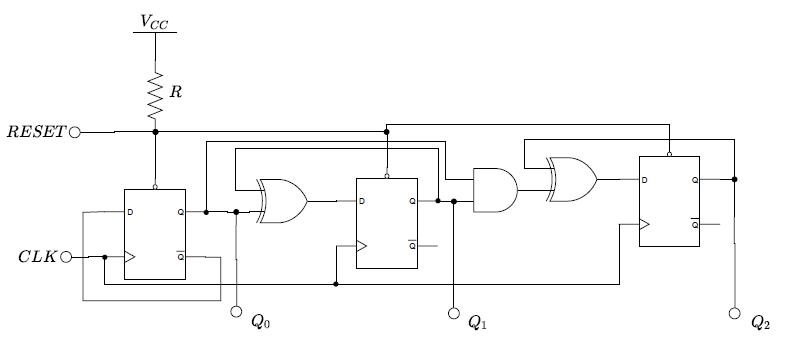
\includegraphics[scale=0.65]{../EJ7/Recursos/contador_sincronico.png}
    \caption{Circuito contador sincr\'onico de 3 bits}
    \label{fig:contador_sincronico_circuito}
\end{figure}

\subsubsection{Dise\~no de PCB}

\begin{figure}[H]
    \centering
        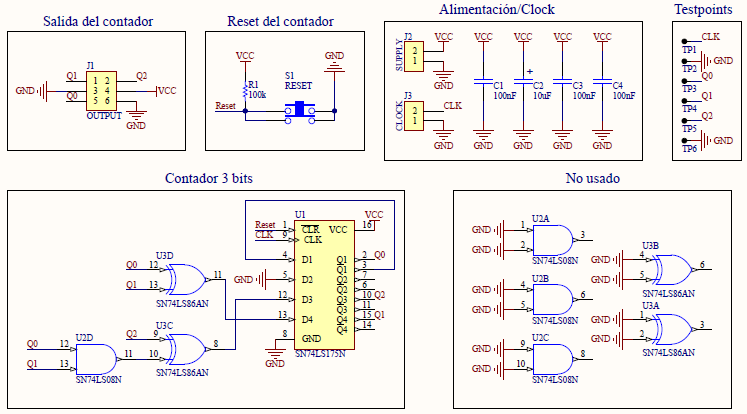
\includegraphics[scale=0.7]{../EJ7/Recursos/esquematico_sincronico.PNG}
    \caption{Esquem\'atico del PCB en Altium Designer}
    \label{fig:esquematico_sincronico}
\end{figure}

\begin{figure}[H]
    \centering
    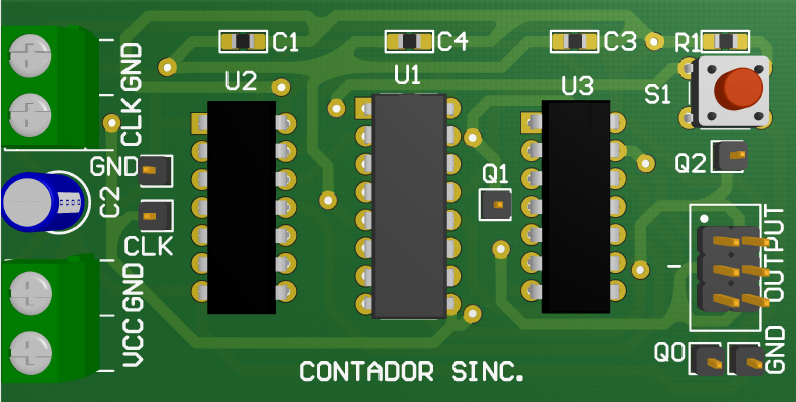
\includegraphics[scale=0.6]{../EJ7/Recursos/3d_top_sincronico.PNG}
    \caption{Dise\~no 3D del PCB}
    \label{fig:3d_sincronico_top}
\end{figure}

\begin{figure}[H]
    \centering
    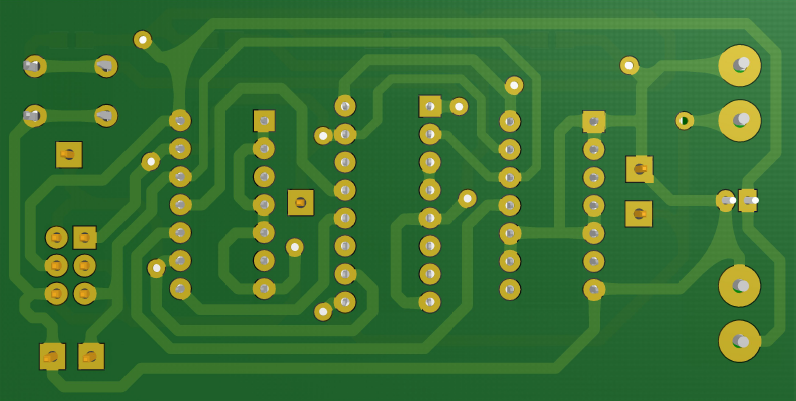
\includegraphics[scale=0.6]{../EJ7/Recursos/3d_bottom_sincronico.PNG} 
    \caption{Dise\~no 3D del PCB}
    \label{fig:3d_sincronico_bottom}
\end{figure}

\subsection{Visualizaci\'on del contador}
Se propone dise\~nar un circuito que decodifique el c\'odigo binario del contador y lo represente en un display
de 7 segmentos para poder realizar una prueba r\'apida del funcionamiento del circuito y poder visualizar el resultado del mismo.

\subsubsection{Dise\~no del circuito}
Se utilizar\'a un circuito integrado 74LS47, esto es, un decodificador BCD a 7 Segmentos, puesto que como la salida del contador se encuentra acotada
entonces puede ser interpretada como BCD. En este integrado la l\'ogica se encuentra negada, por lo cual es necesario utilizar un display de 7 segmentos de \'anodo com\'un,
donde el m\'aximo de corriente que puede entregar es $25mA$, no obstante se har\'a circular una corriente de $4mA$ por segmento teniendo en cuenta que el modelo utilizado tiene una
tensi\'on $V_{D_ON} \approx 2.7V$.

Asumiendo el peor caso donde la tensi\'on sobre la resistencia es m\'axima y puede circular el m\'aximo de corriente, se limita al valor consignado y por ello se utilizan resistencias
de $R = \frac{5V - 2.7V}{4mA} > 575 \Omega \Rightarrow R = 680 \Omega$.

\begin{figure}[H]
    \centering
        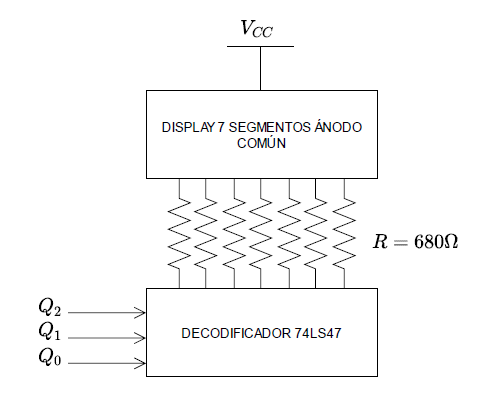
\includegraphics[scale=0.6]{../EJ7/Recursos/visualizacion_simple.png}
    \caption{Simplificaci\'on del circuito de visualizaci\'on}
    \label{fig:visualizacion_simple_circuito}
\end{figure}

\subsubsection{Dise\~no de PCB}

\begin{figure}[H]
    \centering
        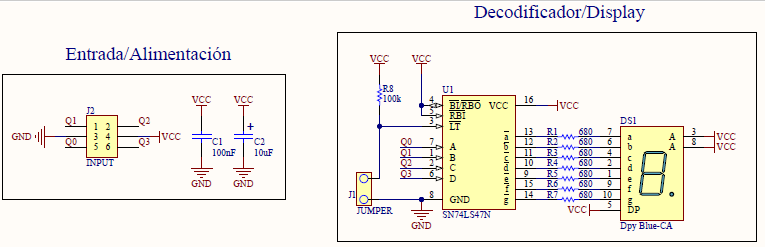
\includegraphics[scale=0.7]{../EJ7/Recursos/esquematico_visualizacion.PNG}
    \caption{Esquem\'atico del PCB en Altium Designer}
    \label{fig:esquematico_visualizacion}
\end{figure}

\begin{figure}[H]
    \centering
    \begin{tabular}{c c}
        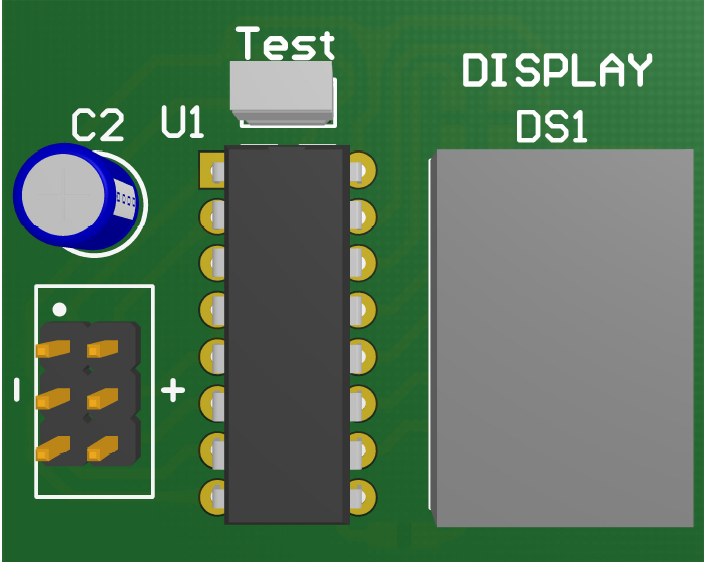
\includegraphics[scale=0.4]{../EJ7/Recursos/3d_top_visualizacion.PNG} &
        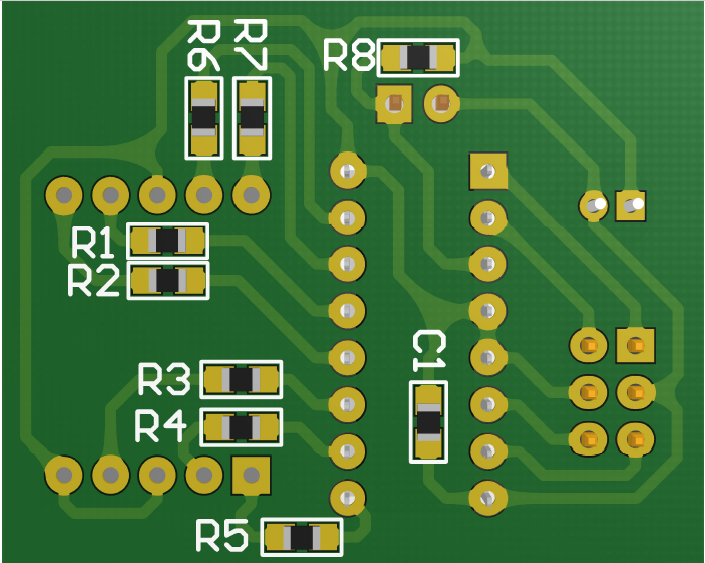
\includegraphics[scale=0.4]{../EJ7/Recursos/3d_bottom_visualizacion.PNG} 
    \end{tabular}
    \caption{Dise\~no 3D del PCB}
    \label{fig:3d_visualizacion}
\end{figure}

\subsection{Resultados}
\subsubsection{Funcionamiento}
\subsubsection{Mediciones}
\subsubsection{An\'alisis de datos}
